\documentclass[a4paper]{article}
\usepackage[portuguese]{babel}
\usepackage[utf8]{inputenc}
\usepackage{indentfirst}
\usepackage{graphicx}
\usepackage{verbatim}
\usepackage{hyperref}
\hypersetup{colorlinks=true, linkcolor=black}
\usepackage{listings}

\begin{document}

\setlength{\textwidth}{16cm}
\setlength{\textheight}{22cm}

\title{\Huge\textbf{Trabalho 2}\linebreak\linebreak\linebreak
\LARGE{Configuração de uma rede e desenvolvimento de uma aplicação de download}\linebreak\linebreak
\Large\textbf{Relatório Final}\linebreak\linebreak

\includegraphics[scale=0.1]{res/feup-logo.png}\linebreak\linebreak\linebreak
\Large{Mestrado Integrado em Engenharia Informática e Computação} \linebreak\linebreak
\Large{Redes de Computadores}
}
\author{\textbf{Professor:}\\ Manuel Ricardo\\\\\textbf{Turma 4:}\\ Henrique Manuel Martins Ferrolho - ei12079 \\ João Filipe Figueiredo Pereira - ei12023 \\ José Pedro Vieira de Carvalho Pinto - ei12164 \\ Miguel Ângelo Jesus Vidal Ribeiro - ei11144\\\linebreak\linebreak \\
 \\ Faculdade de Engenharia da Universidade do Porto \\ Rua Roberto Frias, s\/n, 4200-465 Porto, Portugal \linebreak\linebreak\linebreak
\linebreak\linebreak\vspace{1cm}}
\maketitle
\thispagestyle{empty}

%************************************************************************************************
%************************************************************************************************

\newpage

\section*{Resumo}
Este relatório complementa o segundo projecto da Unidade Curricular de Redes de Computadores, do Mestrado Integrado em Engenharia Informática e de Computação. O projecto consiste na configuração de uma rede de computadores e no desenvolvimento de uma aplicação de download de um ficheiro.
Este documento subdivide-se em diversas secções destacando-se duas delas:

- A secção da aplicação de download onde é descrita a sua arquitectura e apresentados os resultados da sua execução, assim como a sua análise; 

- A secção de configuração da rede onde foi proposto ao grupo a realização de seis experiências tendo cada uma delas objectivos delineados e independentes.\linebreak

As experiências acima referidas basearam-se na configuração de um \textbf{IP de rede}, de um \textbf{router em Linux}, de um \textbf{router comercial} e do \textbf{DNS} (\textit{Domain Name System}), e na implementação de duas \textbf{LAN's} (\textit{Local Area Network}) \textbf{virtuais no switch} e do \textbf{NAT} (\textit{Network Address Translation}) e num teste com a aplicação de download desenvolvida para a verificação de um bom \textbf{funcionamento nas ligações TCP} (\textit{Transmission Control Protocol}). Estes conceitos e funções de protocolos, sistemas e redes, referidos anteriormente, serão explicados mais à frente no relatório.

\newpage

\tableofcontents
\newpage

\section{Introdução}
O segundo projecto de Redes de Computadores desenvolveu-se ao longo de diversas aulas laboratoriais, sendo que a primeira aula serviu para uma maior interiorização acerca de protocolos de aplicação IETF (\textit{Internet Engineering Task Force}). Esta comunidade tem como objectivo proporcionar soluções a problemas relacionados com ligações à \textit{Internet} e para tal são recomendados os documentos RFC (\textit{Request for Comments}) que descrevem padrões de protocolos da mesma.
O protocolo usado no trabalho foi o FTP com auxílio de um servidor da faculdade, a exemplo \textit{ftp.fe.up.pt}, \textit{ftp.up.pt}, entre outros.
Este trabalho visou o estudo de uma rede de computadores, da sua configuração e posterior ligação a uma aplicação desenvolvida pelo grupo. Para tal, além de seguir as recomendações e instruções fornecidas no guião, o grupo teve de fazer pesquisas acerca do funcionamento do protocolo em questão e respectiva ligação ao servidor em uso.

O projecto divide-se em duas grandes componentes: a configuração de uma rede e o desenvolvimento de uma aplicação de download.\linebreak

O principal objectivo da configuração de rede é permitir a execução de uma aplicação, a partir de duas \textit{VLANs} dentro de um \textit{switch}. Numa das VLAN foi implementado o NAT, estando este activo, e na outra não, tendo esta última que conseguir ter ligação à \textit{Internet} para a aplicação de download funcionar correctamente.

Quanto aos objectivos da aplicação de download era essencial o grupo entender o que é um cliente, um servidor e as suas especificidades em TCP/IP, saber como se caracterizam protocolos em aplicações no geral, como definir um \textit{URL} e descrever o comportamento de um servidor FTP. Com estes objectivos concluídos, o grupo poderia avançar para o desenvolvimento da aplicação implementando um cliente FTP e uma ligação TCP a partir de \textit{sockets}. Só então poderiamos concluir a importância do DNS na conversão de um \textit{URL} para um IP, permitindo a sua localização num \textit{host} com domínio determinado.\linebreak

Este relatório divide-se em:

- \textbf{Introdução}, onde são descritos os objectivos do trabalho;

- \textbf{Parte 1 - Aplicação de Download}, onde é descrita a sua arquitectura, apresentados resultados e a sua análise e quais foram os documentos que o grupo utilizou em auxílio na sua implementação;

- \textbf{Parte 2 - Configuração da rede e análise}, onde é descrita a sua arquitectura, objectivos de cada experiência, comandos de configuração e análise dos \textit{logs} gravados durante a sua realização;

- \textbf{Conclusões}, onde são redigidas as últimas análises e opinião final do grupo ao projecto;

- \textbf{Bibliografia}, onde são colocados todos os documentos/\textit{sites} de consulta efectuados pelo grupo;

- \textbf{Anexos}, onde será colocado o código relativo à aplicação, comandos de configuração e \textit{logs} gravados.\linebreak

Antes de prosseguir é de referir que o grupo desenvolveu este projecto em ambiente LINUX, com a linguagem de programação C.

\section{Parte 1 - Aplicação de download}
Uma das componentes do segundo projecto de Redes de Computadores era o desenvolvimento de uma aplicação de download na linguagem de programação C. Para a sua implementação o grupo teve de estudar vários documentos, nomeadamente o RFC959 que aborda o protocolo de transferência de ficheiros (FTP)  e o RFC1738 que informa sobre o uso de \textit{URL's} e o seu devido tratamento.

De seguida iremos descrever resumidamente o plano de implementação do programa e quais as suas funcionalidades, assim como a apresentação de resultados e a sua análise.

\subsection{Arquitetura}
Para implementar a aplicação o grupo decidiu criar duas camadas: a de processamento do URL e a do cliente FTP.
Em cada camada, existe uma estrutura que contém as propriedades necessárias às funções que estas desempenham.\\
A aplicação aceita um \textit{link} como argumento, que deve ser especificado através da linha de comandos. O \textit{link} pode conter um \textit{username} e \textit{password}, ou então nenhum caso se pretenda usar o modo \textit{anonymous}.

\begin{figure}[h!]
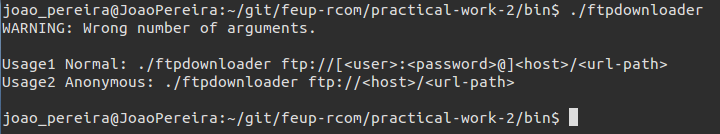
\includegraphics[scale=0.5]{res/usage.png}
\caption{Application usage.}
\end{figure}

A estrutura URL é responsável pelo processamento do argumento especificado na linha de comandos. Esta estrutura contém diversas \textit{strings} que são preenchidas com os diferentes dados presentes no link: \textit{user}, \textit{password}, \textit{hostname}, \textit{path} e \textit{filename}. Após o processamento do URL, o atributo \textit{ip} é preenchido. O atributo \textit{port} é sempre 21 (número da porta de controlo do protocolo FTP).

\begin{figure}[h!]
\centering
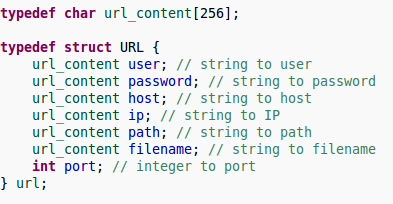
\includegraphics[scale=0.5]{res/url-struct.png}
\caption{URL struct.}
\end{figure}

As funções características desta camada são apresentadas de seguida.
\pagebreak

\begin{figure}[h!]
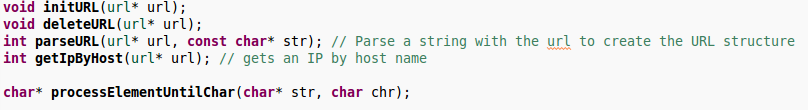
\includegraphics[scale=0.5]{res/url-functions.png}
\caption{URL functions.}
\end{figure}

Breve descrição das funções que constituem esta estrutura:

- \textbf{initURL}, instancia o objecto e aloca memória para os seus atributos;

- \textbf{deleteURL}, liberta a memória alocada anteriormente;

- \textbf{parseURL}, processa o \textit{link} enviado como argumento ao programa e guarda a informação nos respectivos atributos de \textit{url};

- \textbf{getIpByHost}, obtém o IP a partir de um hostname passado como argumento. Este processo deve-se à função \textit{gethostbyname} que retorna uma estrutura do tipo \textit{hostent}, que é usada na função \textit{inet\_ntoa} através de um cast para uma estrutura do tipo \textit{in\_addr} e é devolvido um \textit{char$*$} no formato de números e pontos representando o IP.

A função \textbf{processElementUntilChar} processa uma sub-string até um determinado caracter passado como argumento.\linebreak

No que diz respeito à estrutura do cliente FTP, apenas são necessários dois atributos: um descritor de ficheiro para o socket de controlo e outro para o socket de dados.

\begin{figure}[h!]
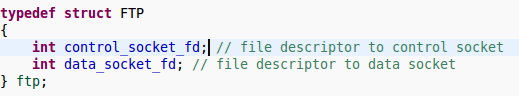
\includegraphics[scale=0.5]{res/ftp-struct.png}
\caption{FTP Client struct.}
\end{figure}

Após o processamento do \textit{URL} estar concluído, é necessário ligar o cliente FTP através de um socket TCP ao servidor em questão, neste caso FTP. Para isso utiliza-se a função \textbf{ftpConnect}. Seguindo o protocolo FTP, e a primeira aula laboratorial, o grupo estabeleceu uma ordem de comandos a enviar que será analisada na apresentação de resultados. A ordem pela qual a comunicação foi feita foi:

 -\textbf{USER user}, o nome do utilizador é enviado;
 
 -\textbf{PASS pass}, onde o utilizador envia a password para o servidor;
 
 -\textbf{CWD path}, permite ao servidor alterar o diretório em que se encontra, indo para aquele onde se encontra o ficheiro;
 
 -\textbf{PASV}, entrada em modo passivo, permitindo uma mútua comunicação entre o servidor e o cliente FTP. É também feita nova conexão do socket mas, desta vez, a uma porta processada com informação recebida do servidor, sendo guardada no descritor de dados do cliente FTP;
 
 -\textbf{RETR filename}, é pedido ao servidor o envio do ficheiro para download.
 
Ao fim de realizados estes passos, inicia-se a transferência do ficheiro especificado pelo utilizador. As funções responsáveis pela comunicação entre o cliente FTP e o servidor apresentam-se de seguida.

\begin{figure}[h!]
\centering
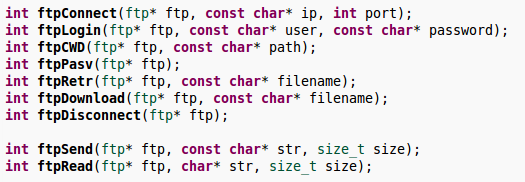
\includegraphics[scale=0.5]{res/ftp-functions.png}
\caption{FTP Client functions.}
\end{figure}

Um ponto importante a frisar na comunicação entre as duas camadas é que o cliente FTP recorre aos atributos do URL previamente formado para executar todas as acções de comunicação e posterior transferência do ficheiro, não existindo mais nenhuma relação entre estas.

\subsection{Resultados de download}
Nesta secção de demonstração e análise de resultados, o grupo decidiu fazer testes em dois modos: normal, com um \textit{username} e \textit{password}, e em anónimo.

Numa primeira análise o grupo irá abordar o modo anónimo com o servidor FTP da Universidade do Porto para o download de um ficheiro escolhido ao acaso.
Para execução do programa faz-se uma introdução do comandos:
\textit{./ftpdownloader ftp://ftp.up.pt/pub/CPAN/RECENT-1M.json} , onde será feito o download do ficheiro RECENT-1M.json.

Para visualizar o resultado da execução na linha de comandos clique -$>$~\autoref{fig:anonymous}

No terminal é possível verificar o pedido de \textit{email} para a entrada em modo anónimo no servidor. De seguida são enviados os comandos ao servidor para uma devida configuração antes do início da transferência. A parte do login do utilizador é assegurada pela função \textbf{\textit{ftpLogin}} do cliente FTP, prosseguida da mudança de directório do servidor com \textbf{\textit{ftpCWD}} para a pasta do ficheiro pretendido. De referir que são sempre recebidas respostas a cada comunicação entre a aplicação e o servidor. Cada mensagem é identificada por três algarismos sendo o primeiro identificador de uma resposta positiva (1-3) ou negativa (4 e 5). O segundo algarismo é de agrupamento e com codificação de informações (0-5). Já o último é um contador para as diferentes mensagens para cada grupo (isto é, dos dois primeiros algarismos; exemplo, 55 nos dois primeiros algarismos terá 4 mensagens do 0 a 4).
De volta à demonstração e após a mudança de directório é feita a entrada em modo passivo por parte da função \textbf{\textit{ftpPasv}}, onde é processada a informação recebida e calculada uma nova porta para a transferência de dados. Na imagem são apresentados os resultados obtidos. Por fim a aplicação pede ao servidor o envio do ficheiro com \textbf{\textit{ftpRetr}} iniciando-se a transferência com \textbf{\textit{ftpDownload}}. Quando a transferência termina é recebida a mensagem \textit{226 File send OK}. O ficheiro recebido tinha tamanho de 2.3 Mb e demorou cerca de 13 segundos. O tempo porém é influenciado com a rede que a aplicação é usada, variando sempre em diferentes execuções.

Para visualizar o resultado transferência clique:

-$>$Antes~\autoref{fig:antesanony}

-$>$Depois~\autoref{fig:depoisanony}

\pagebreak

De seguida apresenta-se a demonstração do download de uma música no modo normal.
Para visualizar a sua execução no terminal clique -$>$~\autoref{fig:normal}

O funcionamento do programa é igual no modo normal e no modo anónimo, sendo a única diferença o \textit{login}. Este em vez de se registar como \textit{anonymous} utiliza as credenciais que o utilizador passa como argumentos da execução.

O tempo registado para a transferência deste ficheiro foi de 15 segundos, com um tamanho de 8.5 Mb. Isto serve para comprovar que o tempo nesta experiência não pode ser tomado como factor preponderante pois a sua resolução não se encontra ao alcance do grupo.

Aqui ficam as imagens relativas a antes e depois da transferência.

-$>$Antes~\autoref{fig:antesnormal}

-$>$Depois~\autoref{fig:depoisnormal}


\section{Parte 2 - Configuração da rede e análise}
\subsection{Experiência 1 - Configurar um IP de rede}
A finalidade desta experiência foi a compreensão da configuração de IP’s em máquinas diferentes, de modo a que estas consigam comunicar entre si. Assim, após a configuração dos IP’s das portas eth0 de dois computadores e a adição das rotas necessárias à tabela de reencaminhamento, foi enviado o sinal “ping” de um computador para o outro, para verificar que, de facto, as máquinas tinham uma ligação entre si.

Para a configuração dos computadores foi utilizado o comando \textbf{\textit{$<$ifconfig [ip]$>$}}, que atribui ao IP da interface o IP passado como argumento. Após esta configuração, executamos um ping de uma máquina para a outra com os IP’s definidos, operação essa que foi executada com sucesso. Foi também possível ver os pedidos ARP, com os pings definidos e a resposta da máquina correspondente com o seu endereço MAC.

\begin{figure}[h!]
\centering
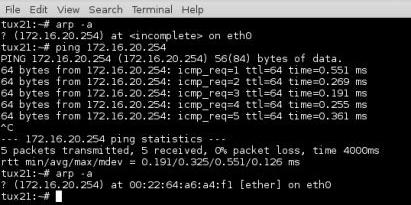
\includegraphics[scale=0.5]{res/image1.jpg}
\caption{Exemplo do output de um \emph{ping}.}
\end{figure}

O ping, após obter o endereço MAC através dos pacotes ARP, gera pacotes do protocolo ICMP. Em frames do tipo Ethernet, os bits vinte e um e vinte e dois do frame identificam o protocolo para o qual deve ser enviado o payload.

\pagebreak

A interface loopback é uma interface de rede virtual que o computador utiliza para comunicar com ele próprio, com o objectivo de realizar testes de diagnóstico, ou aceder a servidores na própria máquina, como se fosse um cliente. Assim, uma interface loopback, permite a existência de um endereço IP no router, que está sempre activo, em vez de ser dependente de uma interface física.

\subsection{Experiência 2 - Implementar duas LAN's virtuais no switch}
Nesta experiência foram criadas duas LANs virtuais no switch: a primeira constituída pelas máquinas 1 e 4, e a segunda pela máquina 2. Com esta configuração, a máquina 2 deixaria de ter acesso ás maquinas 1 e 4, uma vez que se encontrariam em sub-redes diferentes.

Para a configuração do switch foi necessário entrar na sua consola de configuração e executar o comando \textbf{\textit{$<$vlan [n]$>$}}, onde \textbf{\textit{n}} é o número identificador da VLAN. Após a configuração das VLANs foi necessário adicionar as portas do switch às respectivas VLANs, para criar duas sub-redes individuais. Para isso usaram-se os comandos \textbf{\textit{$<$interface fastethernet 0/[i]$>$}}, onde \textbf{\textit{i}} é o identificador da porta do switch, seguido de \textbf{\textit{$<$switchport mode access$>$}} e \textbf{\textit{$<$switchport access VLAN [n]$>$}} onde \textit{\textbf{n}} é o identificador da VLAN criada.

\begin{figure}[h!]
\centering
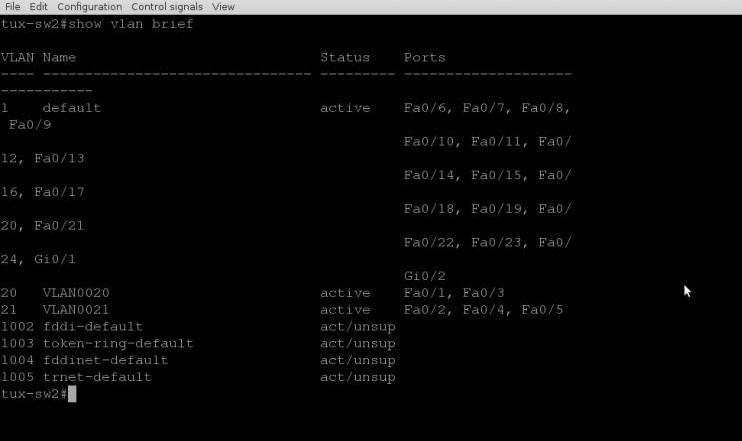
\includegraphics[scale=0.3]{res/image3.jpg}
\caption{Output do briefing da VLAN.}
\end{figure}

Após estas configurações foi executado um ping para a máquina 2 que, tal como esperado, falhou, uma vez que se encontrava numa sub-rede diferente, inacessível tanto pela máquina 1, como pela máquina 4.

\subsection{Experiência 3 - Configurar um router em Linux}
O objectivo desta experiência era configurar a máquina 4 como router entre as duas sub-redes criadas na experiência dois.\\
Para realizar esta tarefa, foi necessário ligar a interface ethernet 1 da máquina 4 e configurá-la com um IP dentro da mesma gama que a máquina 2, e adicionar esta interface à sub-rede da máquina 2.\\
Após esta configuração, adicionou-se uma rota à máquina 1 utilizando o comando \textbf{\textit{$<$route add –net  172.16.y1.0/24 gw 172.16.y0.254$>$}}. O primeiro endereço identifica a gama de endereços para a qual se quer adicionar a rota; o segundo endereço identifica o IP para o qual se deve reencaminhar o pacote (neste caso o IP da máquina 4). Posteriormente, repetiu-se o mesmo procedimento para a máquina 2, mas utilizando os seguintes endereços \textbf{\textit{$<$route add –net 172.16.y0.0/24 gw 172.16.y1.253$>$}}. Novamente, o IP 172.16.y1.253, é o IP da máquina 4 nesta sub-rede.\\
Finalmente, foi possível \emph{pingar} a máquina 2 a partir da máquina 1. O pedido para o IP da máquina 2 - 172.16.y1.1 -, é reencaminhado para a máquina 4 - 172.16.y0.254; como a máquina 4 está ligada à sub-rede de ambas as máquinas, consegue aceder à máquina 2 - 172.16.y1.1 -, através da sua interface eth1, que está nessa sub-rede, e assim reencaminha o pacote para a máquina 2. Na resposta, o processo é idêntico, sendo o pacote reencaminhado da máquina 2, para a máquina 1.


\subsection{Experiência 4 - Configurar um router comercial e implementar o NAT}
Nesta experiência pretendia-se que fosse configurado um router comercial com NAT devidamente implementado. A implementação do NAT (Network Adress Translation) teve como objectivo possibilitar a comunicação entre os computadores da rede criada com redes externas. Por se tratar de uma rede privada, os ip’s nunca seriam reconhecidos fora da rede. Por isso, criou-se uma técnica que permite reescrever os IP’s de origem  de uma rede interna, para que possam aceder a uma rede externa. Este procedimento gera um número de 16 bits, utilizando esse valor numa hash table, e escrevendo-o no campo da porta de origem. Na resposta, o processo é revertido, e o router sabe para qual computador da rede interna deve enviar a resposta.\\
Para configurar o router, foi necessário configurar a interface interna no processo de NAT. Para isso, entrou-se na consola de configuração da interface fastethernet 0/0 do router, com o comando \textbf{\textit{$<$interface fastethernet 0/0$>$}}. Em adição, teve de ser especificado qual o IP para essa interface, introduzindo o comando\textbf{ \textit{$<$ ip address [ip] [mask] $>$}}, onde, neste caso, o \textbf{\textit{ip}} correspondeu ao 172.16.21.254, e a \textbf{\textit{mask}} a 255.255.255.0.\\
Posteriormente, foi configurada a interface externa, atribuindo um IP à interface 1, que estava ligada ao router da sala. Para isso, introduziram-se os seguintes comandos: \textbf{\textit{$<$interface fastethernet 0/1$>$}}, \textbf{\textit{$<$ip adress 172.16.1.29 255.255.255.0$>$}}. Para ambos os casos foi necessário introduzir o comando \textbf{\textit{$<$no shutdown$>$}}, para que estas configurações se mantivessem caso o router fosse desligado.\\
De seguida, para que fosse garantida a gama de endereços, introduziram-se os comandos: \textbf{\textit{$<$ip nat pool ovrld 172.16.1.29 172.16.1.29 prefix 24$>$}} e \textbf{\textit{$<$ip nat inside source list 1 pool ovrld overload$>$}}.\\
Posteriormente, foi criada uma lista de acessos e permissões de pacotes, para cada uma das sub-redes, com o comando \textbf{\textit{$<$acesslist 1 permit ip [máximo]$>$}}. Neste caso, o IP utilizado foi 172.16.20.0 e 172.16.21.0, que poderia ir até 172.16.2X.255, colocando 0.0.0.255 no campo \textbf{\textit{máximo}}.\\
Finalmente, foram definidas as rotas internas e externas, aplicando \textbf{\textit{$<$ip route 0.0.0.0
0.0.0.0 172.16.1.254$>$}} e \textbf{\textit{$<$ip route 172.16.20.0 255.255.255.0 172.16.21.253$>$}}, este comando cria uma rota, quando o IP de destino for 172.16.20.0-255 deve redireccionar os pacotes para o IP 172.16.21.253.
Para testar, foi executado na máquina 1 um ping ao router da sala e verificou-se que os pacotes enviados para a máquina 1, passavam pela máquina 2, onde eram reencaminhados para o router no IP 172.16.21.254.

\subsection{Experiência 5 - DNS}
O objectivo desta experiência era conseguir aceder a redes externas, conseguindo desta forma aceder à Internet, através da rede interna criada. Para isto, foi necessário configurar o DNS. 

Esta configuração passa por, em todos os hosts da rede criada, aceder e editar o ficheiro resolv.conf. Este ficheiro é lido cada vez que são invocadas rotinas que fornecem acesso à Internet. Neste caso, o ficheiro foi editado colocando \textbf{\textit{“nameserver 172.16.1.1”}}, que se trata do endereço IP do servidor que deve ser acedido.	

\begin{figure}[h!]
\centering
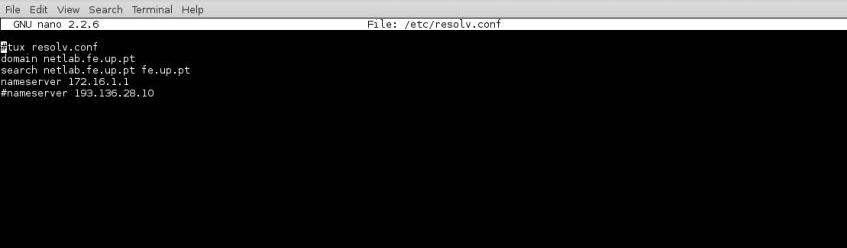
\includegraphics[scale=0.5]{res/image4.jpg}
\end{figure}

Para testar esta experiência, foi feito o teste de ping usando \emph{www.google.com}.\\
Nos logs, consequentemente, verificou-se que o DNS pergunta a informação contida num dado domain name, e este responde com o tempo de vida e o tamanho do pacote de dados.\linebreak
Exemplo:

Query-$>$ www.google.com: Type A, class IN.

Answer-$>$ Name: www.google.com, Type: A, Class: IN, Time to live: 39.

seconds, Data Length: 4, Addr: 173.194.41.206

\subsection{Experiência 6 - Ligações TCP}
Por fim, na experiência 6, compilou-se e executou-se a aplicação desenvolvida e descrita na primeira parte do relatório.\\
Para testar a aplicação, foi usado um servidor ftp e efectuado o download de um ficheiro. O download efectuou-se correctamente, o que demonstrou que a rede estava bem configurada, não trazendo qualquer problema no acesso por protocolo ftp, assim como à utilização de um servidor exterior à rede.

TCP utiliza \textit{Selective Repeat ARQ}, que é semelhante ao \textit{GO-BACK-N ARQ}, com a diferença que o receptor não deixa de processar os frames recebidos quando detecta um erro. Quando falha de um frame é detectada, o receptor continua um \textit{acknowledgement} com o número da frame que falhou. O receptor continua a receber e a processar as frames seguintes, enviando sempre, no \textit{ack}, o número da frame que falhou primeiro. No final do envio, o emissor verifica os \textit{ack} e reenvia os frame perdidos.

\section{Conclusões}
Após a conclusão do segundo projecto de Redes e Computadores, o grupo interiorizou não todos mas os conceitos necessários para uma estável e coerente implementação do que era pedido no guião.

\hfill

A configuração de rede foi concluída com sucesso permitindo a todos os elementos do grupo uma possível implementação ou, pelo menos, ter uma noção de como tudo funciona e assim aplicar esta prática a nível profissional.

A aplicação de download embora fosse mais fácil de implementar, implicava um prévio estudo de alguns protocolos como os que são descritos nos RFC959 e RFC1738 sobre FTP e sintax do URL, respectivamente.

Todos os objectivos delineados pelo grupo foram atingidos com sucesso. É importante obter conhecimentos acerca de protocolos de ligação pois são bastante utilizados no quotidiano, fornecendo ao grupo uma perspectiva do que é trabalhar no ramo e do que é possível produzir com estas ferramentas.

\hfill

O relatório é sinónimo do término do projecto estando o grupo orgulhoso do que conseguiu produzir.

\clearpage
\addcontentsline{toc}{section}{Referências}
\renewcommand\refname{Referências}
\bibliographystyle{plain}
\begin{thebibliography}{5}
  \bibitem{notes} Manuel Ricardo {\em Lab 2 - Computer Networks.}  2014 \href{http://moodle.up.pt/pluginfile.php/120587/mod_resource/content/3/lab2.pdf}{link}.

  \bibitem{notes} J. Postel, J. Reinolds {\em File Transfer Protocol} 1985 \href{https://www.ietf.org/rfc/rfc959.txt}{link}.

  \bibitem{notes} T. Berners-Lee {\em Uniform Resource Locators} 1994 \href{https://www.ietf.org/rfc/rfc1738.txt}{link}

  \bibitem{notes} Brian Hall {\em Beej's Guide to Network Programming - Using Internet Sockets} 2012 \href{http://www.beej.us/guide/bgnet/output/html/multipage/}{link}

  \bibitem{notes} {\em O Protocolo FTP} 2014 \href{  http://pt.kioskea.net/contents/265-o-protocolo-ftp-file-transfer-protocol}{link}
\end{thebibliography}

\newpage
\appendix
\section{Anexos}
\subsection{Imagens relativas a secções do relatório}

\begin{figure}[h!]
\centering
\caption{Demonstração - Modo Anónimo}
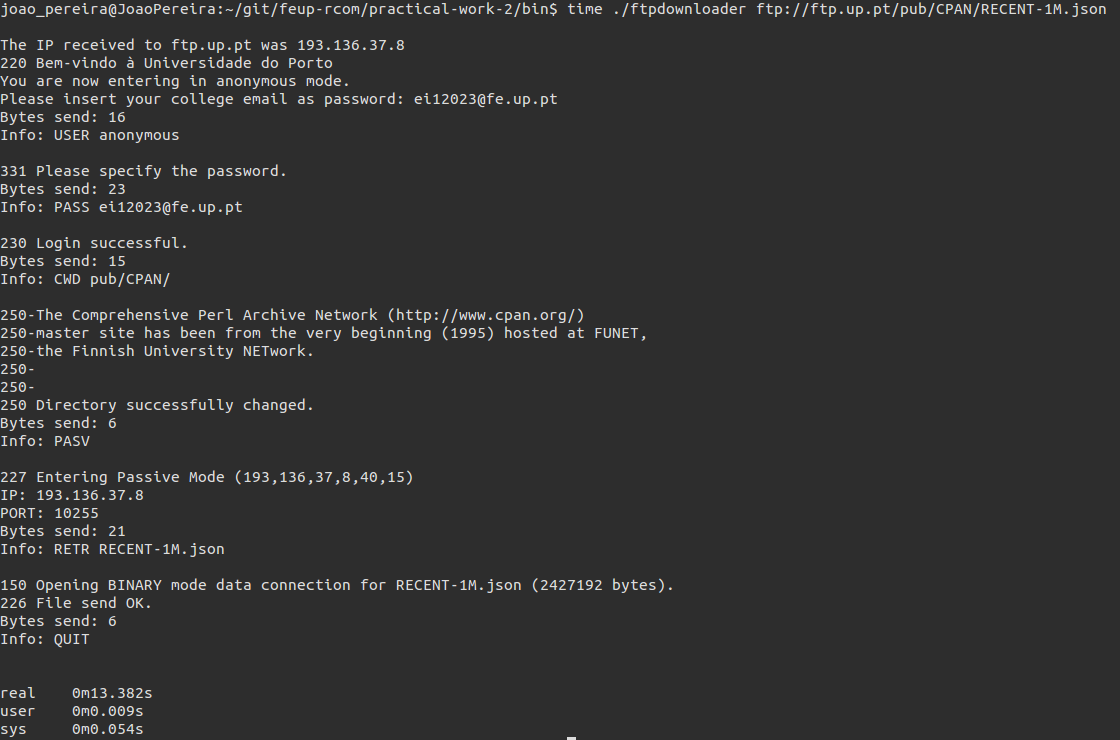
\includegraphics[scale=0.3]{res/teste-anonymous.png}
\label{fig:anonymous}
\end{figure}

\begin{figure}[h!]
\centering
\caption{Modo anónimo - antes}
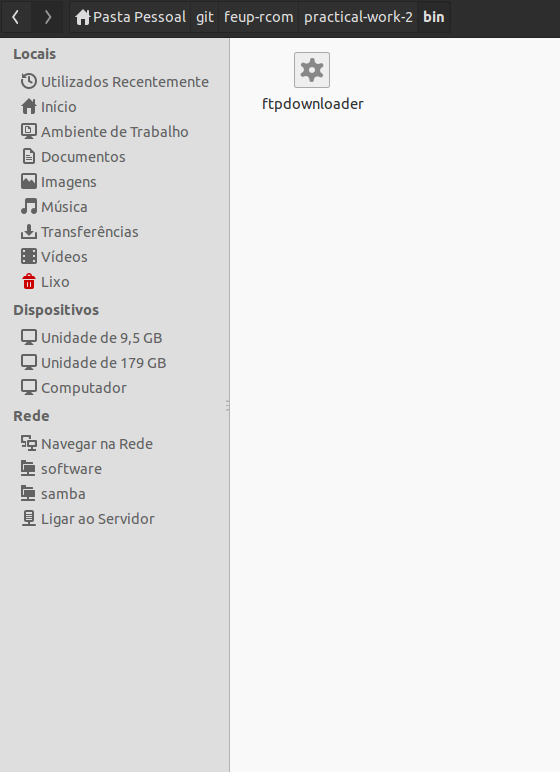
\includegraphics[scale=0.35]{res/antes-modoanonimo.png}
\label{fig:antesanony}
\end{figure}

\begin{figure}[h!]
\centering
\caption{Modo anónimo - depois}
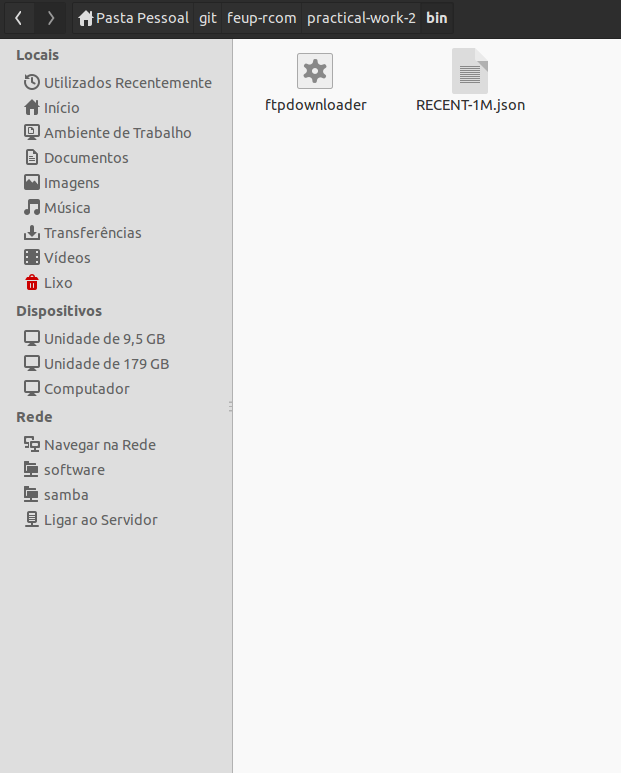
\includegraphics[scale=0.35]{res/depois-modoanonimo.png}
\label{fig:depoisanony}
\end{figure}

\pagebreak

\begin{figure}[h!]
\centering
\caption{Demonstração - Modo Normal}
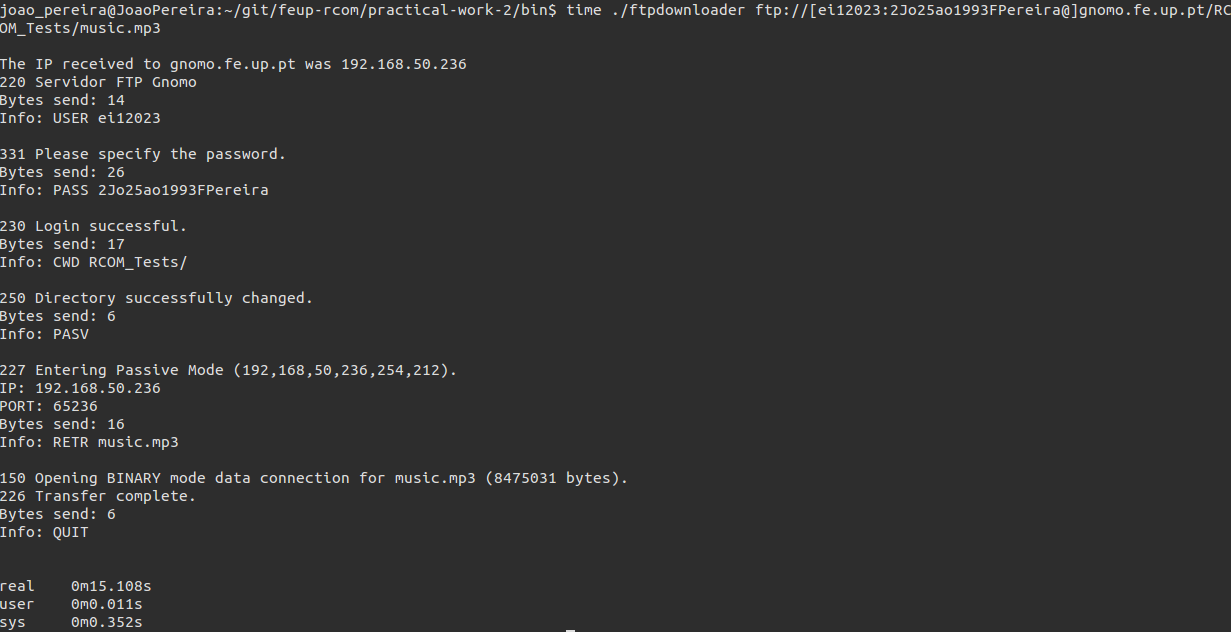
\includegraphics[scale=0.3]{res/teste-normal.png}
\label{fig:normal}
\end{figure}

\pagebreak

\begin{figure}[h!]
\centering
\caption{Modo normal - antes}
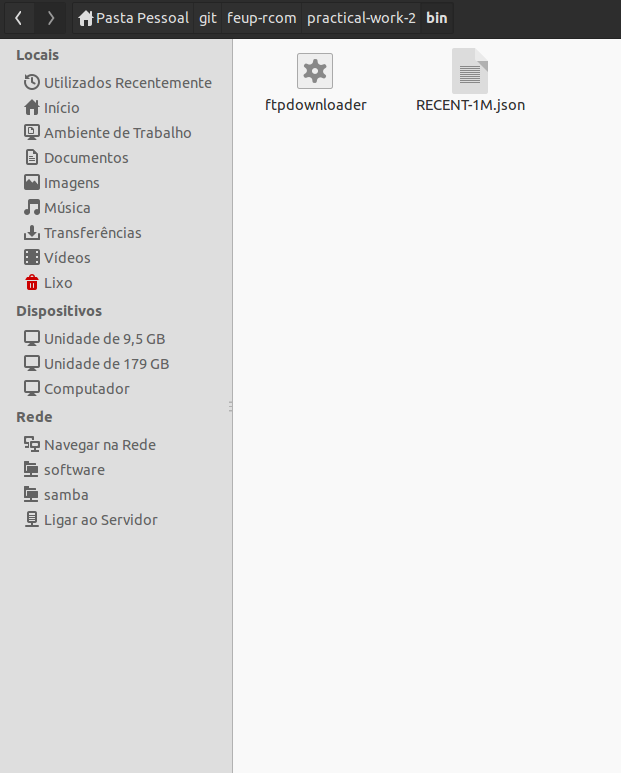
\includegraphics[scale=0.35]{res/depois-modoanonimo.png}
\label{fig:antesnormal}
\end{figure}

\begin{figure}[h!]
\centering
\caption{Modo normal - depois}
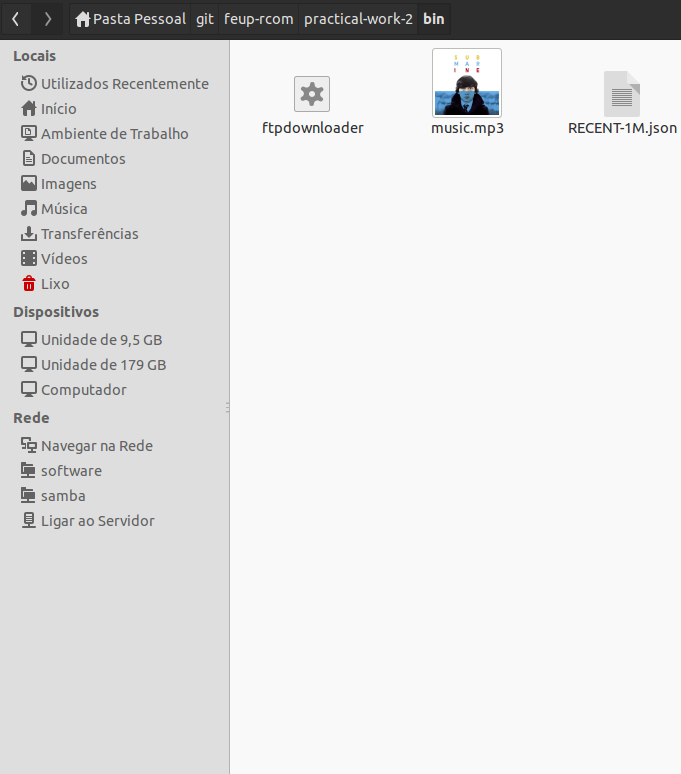
\includegraphics[scale=0.35]{res/depois-modonormal.png}
\label{fig:depoisnormal}
\end{figure}

\subsection{Código da aplicação}
\newenvironment{changemargin}[2]{%
\begin{list}{}{%
\setlength{\topsep}{0pt}%
\setlength{\leftmargin}{#1}%
\setlength{\rightmargin}{#2}%
\setlength{\listparindent}{\parindent}%
\setlength{\itemindent}{\parindent}%
\setlength{\parsep}{\parskip}%
}%
\item[]}{
\end{list}}

{\underline{\textit{\textbf{Main.c}}}}

\begin{changemargin}{-3cm}{-4cm}
{\small\lstinputlisting[language=C]{src/Main.c}}
\end{changemargin}

{\underline{\textit{\textbf{URL.h}}}}

\begin{changemargin}{-3cm}{-4cm}
{\small\lstinputlisting[language=C]{src/URL.h}}
\end{changemargin}

{\underline{\textit{\textbf{URL.c}}}}

\begin{changemargin}{-3cm}{-4cm}
{\small\lstinputlisting[language=C]{src/URL.c}}
\end{changemargin}

{\underline{\textit{\textbf{FTP.h}}}}

\begin{changemargin}{-3cm}{-4cm}
\lstinputlisting[language=C]{src/FTP.h}
\end{changemargin}

{\underline{\textit{\textbf{FTP.c}}}}

\begin{changemargin}{-3cm}{-4cm}
{\small\lstinputlisting[language=C]{src/FTP.c}}
\end{changemargin}

\pagebreak

\subsection{Comandos de configuração}
{\underline{\textit{\textbf{Experiência 1 - Configurar um IP de rede}}}}
\obeylines
\input{exp/exp1.txt}

\hfill

{\underline{\textit{\textbf{Experiência 2 - Implementar duas VLANs virtuais no switch}}}}
\obeylines
\input{exp/exp2.txt}

\hfill

{\underline{\textit{\textbf{Experiência 3 - Configurar um router em Linux}}}}
\obeylines
\input{exp/exp3.txt}

\hfill

{\underline{\textit{\textbf{Experiência 4 - Configurar um router comercial e implementar o NAT}}}}
\obeylines
\input{exp/exp4.txt}

\pagebreak

\subsection{Logs gravados}
\begin{figure}[h!]
\caption{Experiência 1 - WireShark}
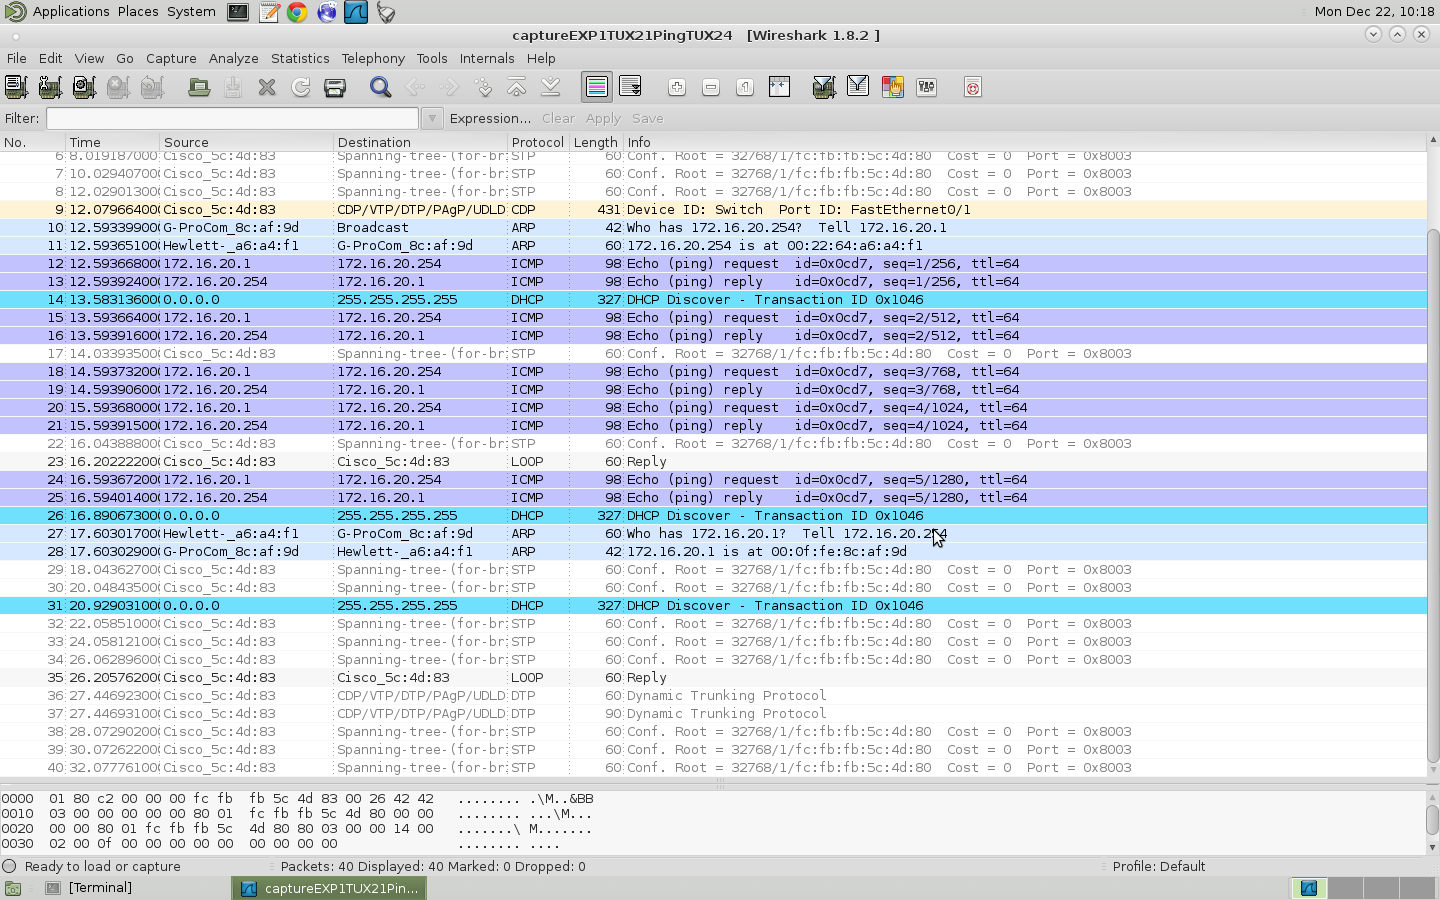
\includegraphics[scale=0.25]{res/image2.png}
\label{fig:teste}
\end{figure}

\end{document}
